%% ID: transfer_energy_ZMF
%% TITLE: Transfer of Energy in Collisions
%% TYPE: question
%% QUESTIONTYPE: numeric
%% CONCEPTS:  energy, momentum, zero_momentum_frame, vectors
%% VIDEOS: 
%% LEVEL: 6
%% TOPIC: mechanics/dynamics
%% ORDER: 7

%\input{../../../Templates/Problem_Template}
%\begin{document}
\begin{problem}[Transfer of Energy in Collision] %A2-2
 {A particle of mass $m_{1}$ and velocity $v$ makes an elastic, head-on collision with a stationary particle of mass $m_{2}$.  Find the velocity of the zero momentum frame relative to the laboratory frame.  By considering the collision in the zero momentum frame, show that in the laboratory frame the fraction of the initial kinetic energy transferred to $m_{2}$ is given by
 \begin{equation}
  \frac{4m_{1}m_{2}}{(m_{1}+m_{2})^{2}}.
 \end{equation}
Three balls of masses $m_{1}$, $m_{2}$ and $m_{3}$ are suspended in a horizontal line by light wires and are almost touching.  The mass $m_{1}$ is given a horizontal velocity $v$ so that it collides head-on with the mass $m_{2}$.  Find an expression for the final kinetic energy of $m_{3}$, and sketch it as a function of $m_{2}$.  What value of $m_{2}$ results in the maximum energy transfer to the mass $m_{3}$?}
{\textit{Cambridge University Tripos 2004}}
{
To find the velocity of the zero momentum frame, which we will call $u$, we consider the total momentum of the system, which is $m_1 v$ and the total mass, $m_1 + m_2$. From this we can say that the centre of mass of the system is moving at $u=\frac{m_1 v}{m_1 + m_2}$ in the same direction as particle 1. This is the velocity of the zero momentum frame and hence we may write the velocities of the two particles as $v-u$ and $-u$ respectively, as shown in Figure \ref{fig:Tripos_Elastic_ZMF_1}.

\begin{figure}[h]
	\centering
	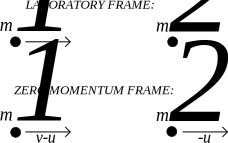
\includegraphics[width=0.5\textwidth]{../../../figures/Tripos_Elastic_ZMF_1.svg}
	\caption{}
	\label{fig:Tripos_Elastic_ZMF_1}
\end{figure}

Now consider the collision between the two particles in the zero momentum frame. Let particles 1 and 2 have final velocities $v_1$ and $v_2$ after the collision in the zero momentum frame. By conservation of linear momentum, the total momentum of the particles in the zero momentum frame must still be zero. This gives us:

\begin{equation*}m_1 v_1 + m_2 v_2=0\end{equation*}
\begin{equation}v_1=-\frac{m_2}{m_1}v_2\end{equation}

Since we are told that the collision is elastic, we may also conserve kinetic energy in the zero momentum frame:

\begin{equation*}\frac{1}{2}m_1 (v-u)^2+\frac{1}{2}m_2(-u)^2=\frac{1}{2}m_1{v_1}^2+\frac{1}{2}m_2{v_2}^2\end{equation*}

Rewriting $v-u$ as $\frac{m_2 v}{m_1 + m_2}$ and substituting our value of $v_1$ from equation 2 into the above equation we find:

\begin{equation*}\frac{1}{2}m_1 \left(\frac{m_2 v}{m_1 + m_2}\right)^2+\frac{1}{2}m_2\left(-\frac{m_1 v}{m_1 + m_2}\right)^2=\frac{1}{2}m_1\left({-\frac{m_2}{m_1}v_2}\right)^2+\frac{1}{2}m_2{v_2}^2\end{equation*}
Expanding out this equation and simplifying we find:

\begin{equation*}v_2=\frac{m_1}{m_1 + m_2}v\end{equation*}

We have taken the positive root of the equation since a negative velocity for $v_2$ would require the particles to pass through each other which is not possible. 

We can now calculate the kinetic energy of particle 2 in the laboratory frame remembering that the zero momentum frame is travelling at a velocity $u$.

\begin{equation*}K.E._{2final}=\frac{1}{2}m_2\left(v_2 + u\right)^2=\frac{1}{2}m_2\left(\frac{m_1v}{m_1 + m_2}+ \frac{m_1 v}{m_1 + m_2}\right)^2=\frac{2{m_1}^2m_2v^2}{\left(m_1 + m_2\right)^2}\end{equation*}

To show what fraction of the total initial kinetic energy this is, we simply divide by the initial kinetic energy in the laboratory frame, which is $\frac{1}{2}m_1v^2$:

\begin{equation}energy fraction=\left(\frac{2{m_1}^2m_2v^2}{\left(m_1 + m_2\right)^2}\right)/\left(\frac{1}{2}m_1v^2\right)=\frac{4m_{1}m_{2}}{(m_{1}+m_{2})^{2}}\end{equation}

For the next part of the question we do not need to consider any further collisions since we have a general formula for the energy fraction passed on to a particle which is initially stationary and then hit by a moving particle. We have shown that this fraction is independent of the velocity of the incoming particle and only depends on the two particles' masses. Therefore we use equation 3 for the second collision between the last two particles just as we did for the first collision, only relabelling the masses appropriately:

\begin{equation*}final~energy~fraction=first~collision~energy~fraction \times second~collision~energy~fraction\end{equation*}
\begin{equation*}final~energy~fraction=\frac{4m_{1}m_{2}}{(m_{1}+m_{2})^{2}}\times \frac{4m_{2}m_{3}}{(m_{2}+m_{3})^{2}}\end{equation*}

Since the initial kinetic energy is simply that of the first particle, the kinetic energy of the final particle after both collisions have occurred is:

\begin{equation*}K.E._{3final}=\frac{1}{2}m_1v^2 \times \frac{4m_{1}m_{2}}{(m_{1}+m_{2})^{2}}\times \frac{4m_{2}m_{3}}{(m_{2}+m_{3})^{2}}=\frac{8{m_{1}}^2{m_{2}}^2m_3v^2}{(m_{1}+m_{2})^{2}(m_{2}+m_{3})^{2}}\end{equation*}

To plot this function we must consider the value in the limit of very small and very large $m_2$. As $m_2 \to 0$ the denominator remains finite while the numerator goes to 0. Therefore the value of the final particle's kinetic energy goes to zero as the mass of the middle particle goes to zero. We must also consider its kinetic energy as $m_2 \to \infty$. Since the numerator goes like ${m_2}^2$ and the denominator goes like ${m_2}^4$, the function goes to zero in this limit. Therefore we expect a maximum at some value of $m_2$. Careful differentiation at $m_2=0$ also shows that the gradient must go to zero here. See Figure \ref{fig:Tripos_Elastic_ZMF_2} for the plot. 

\begin{figure}[h]
	\centering
	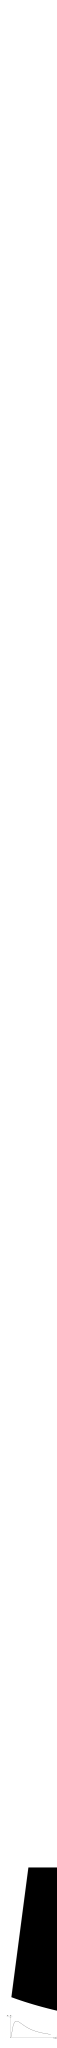
\includegraphics[width=0.7\textwidth]{../../../figures/Tripos_Elastic_ZMF_2.svg}
	\caption{}
	\label{fig:Tripos_Elastic_ZMF_2}
\end{figure}

We finally have to find what value of $m_2$ maximises the third particle's final kinetic energy. This corresponds to the peak of the function in Figure \ref{fig:Tripos_Elastic_ZMF}. To maximise this function, it is easiest to find the minimum of its reciprocal, which is equivalent to finding the minimum of the square root of the reciprocal, and so, ignoring the constants we find the stationary point of the reciprocal as follows:

\begin{equation*}\frac{d}{d{m_2}}\left(\frac{(m_{1}+m_{2})^{2}(m_{2}+m_{3})^{2}}{{m_{2}}^2}
\right)=\frac{d}{d{m_2}}\left(\frac{(m_{1}+m_{2})(m_{2}+m_{3})}{{m_{2}}}
\right)=0\end{equation*}
\begin{equation*}m_2\left(m_1 + m_2 + m_2 +m_3\right)-\left(m_{1}+m_{2})(m_{2}+m_{3}
\right)=0\end{equation*}
\begin{equation*}{m_2}^2=m_1m_3\end{equation*}
\begin{equation*}m_2=\sqrt{m_1m_3}\end{equation*}

And so we find that for the maximum energy transfer to $m_3$ we should choose $m_2=\sqrt{m_1m_3}$.
}
\end{problem}
%\end{document}